% Generated by misc/paper_b/tools/build_figures.py from NUMBERS_TABLE.csv. Do not edit.
% Trust rank agreement and distance to survey distributions by route (descriptive)
\documentclass[border=3pt]{standalone}
\usepackage[T1]{fontenc}
\usepackage{lmodern,amsmath,xcolor}
\usepackage{tikz}
\pdftrailerid{}
\definecolor{cA}{HTML}{0072B2}% blue
\definecolor{cB}{HTML}{D55E00}% vermillion
\definecolor{cC}{HTML}{009E73}% green
\definecolor{cD}{HTML}{CC79A7}% purple
\definecolor{cG}{HTML}{6B6B6B}% grey
\definecolor{cS}{HTML}{3A3A3A}
\definecolor{zebra}{HTML}{F1F1F1}
\definecolor{gridc}{HTML}{C8C8C8}
\newcommand{\Px}{0}\newcommand{\Pmin}{0}\newcommand{\Psc}{1}
% \setpanel{x0 cm}{data value at x0}{cm per data unit}: every data x below is x0 + (v - vmin) * scale.
\newcommand{\setpanel}[3]{\renewcommand{\Px}{#1}\renewcommand{\Pmin}{#2}\renewcommand{\Psc}{#3}}
\newcommand{\XX}[1]{\fpeval{\Px+((#1)-(\Pmin))*\Psc}}
% markers: o filled circle, s filled square, d hollow diamond, t filled triangle, h hollow circle, q hollow square
\newcommand{\mk}[4]{% style colour x y
  \ifx#1o\fill[#2] (#3,#4) circle (0.095);\fi
  \ifx#1h\draw[#2,fill=white,line width=0.7pt] (#3,#4) circle (0.095);\fi
  \ifx#1s\fill[#2] (#3-0.088,#4-0.088) rectangle (#3+0.088,#4+0.088);\fi
  \ifx#1q\draw[#2,fill=white,line width=0.7pt] (#3-0.085,#4-0.085) rectangle (#3+0.085,#4+0.085);\fi
  \ifx#1d\draw[#2,fill=white,line width=0.7pt] (#3,#4+0.125)--(#3+0.125,#4)--(#3,#4-0.125)--(#3-0.125,#4)--cycle;\fi
  \ifx#1t\fill[#2] (#3,#4+0.115)--(#3+0.105,#4-0.085)--(#3-0.105,#4-0.085)--cycle;\fi}
% interval with point: claim, lo, value, hi, y, style, colour, dash(solid|dashed)
\newcommand{\ival}[8]{%
  \edef\xl{\XX{#2}}\edef\xv{\XX{#3}}\edef\xh{\XX{#4}}%
  \draw[#7,line width=0.8pt,#8] (\xl,#5)--(\xh,#5);
  \draw[#7,line width=0.8pt] (\xl,#5-0.055)--(\xl,#5+0.055);
  \draw[#7,line width=0.8pt] (\xh,#5-0.055)--(\xh,#5+0.055);
  \mk{#6}{#7}{\xv}{#5}}
% point only
\newcommand{\pval}[5]{\edef\xv{\XX{#2}}\mk{#4}{#5}{\xv}{#3}}
% stem from the panel zero to the value, with marker: claim, value, y, style, colour
\newcommand{\lval}[5]{\edef\xv{\XX{#2}}\edef\xz{\XX{0}}%
  \draw[#5,line width=0.8pt] (\xz,#3)--(\xv,#3);\mk{#4}{#5}{\xv}{#3}}
% vertical reference line at a data value: claim, value, y0, y1, colour
\newcommand{\vref}[5]{\edef\xv{\XX{#2}}\draw[#5,dashed,line width=0.8pt] (\xv,#3)--(\xv,#4);}
% a printed number tied to a table cell: claim, field, printed, prefix, suffix, x, y, anchor, background fill
\newcommand{\lbl}[9]{\node[anchor=#8,fill=#9,inner sep=1pt,font=\footnotesize] at (#6,#7) {#4#3#5};}
% a printed value with its interval: claim, printed value, printed lo, printed hi, x, y, anchor
\newcommand{\lblci}[7]{\node[anchor=#7,inner sep=0pt,font=\footnotesize] at (#5,#6) {#2\,[#3, #4]};}
% free text (no data)
\newcommand{\txt}[4]{\node[anchor=#3,inner sep=0pt,font=#4] at (#1) {#2};}
\begin{document}
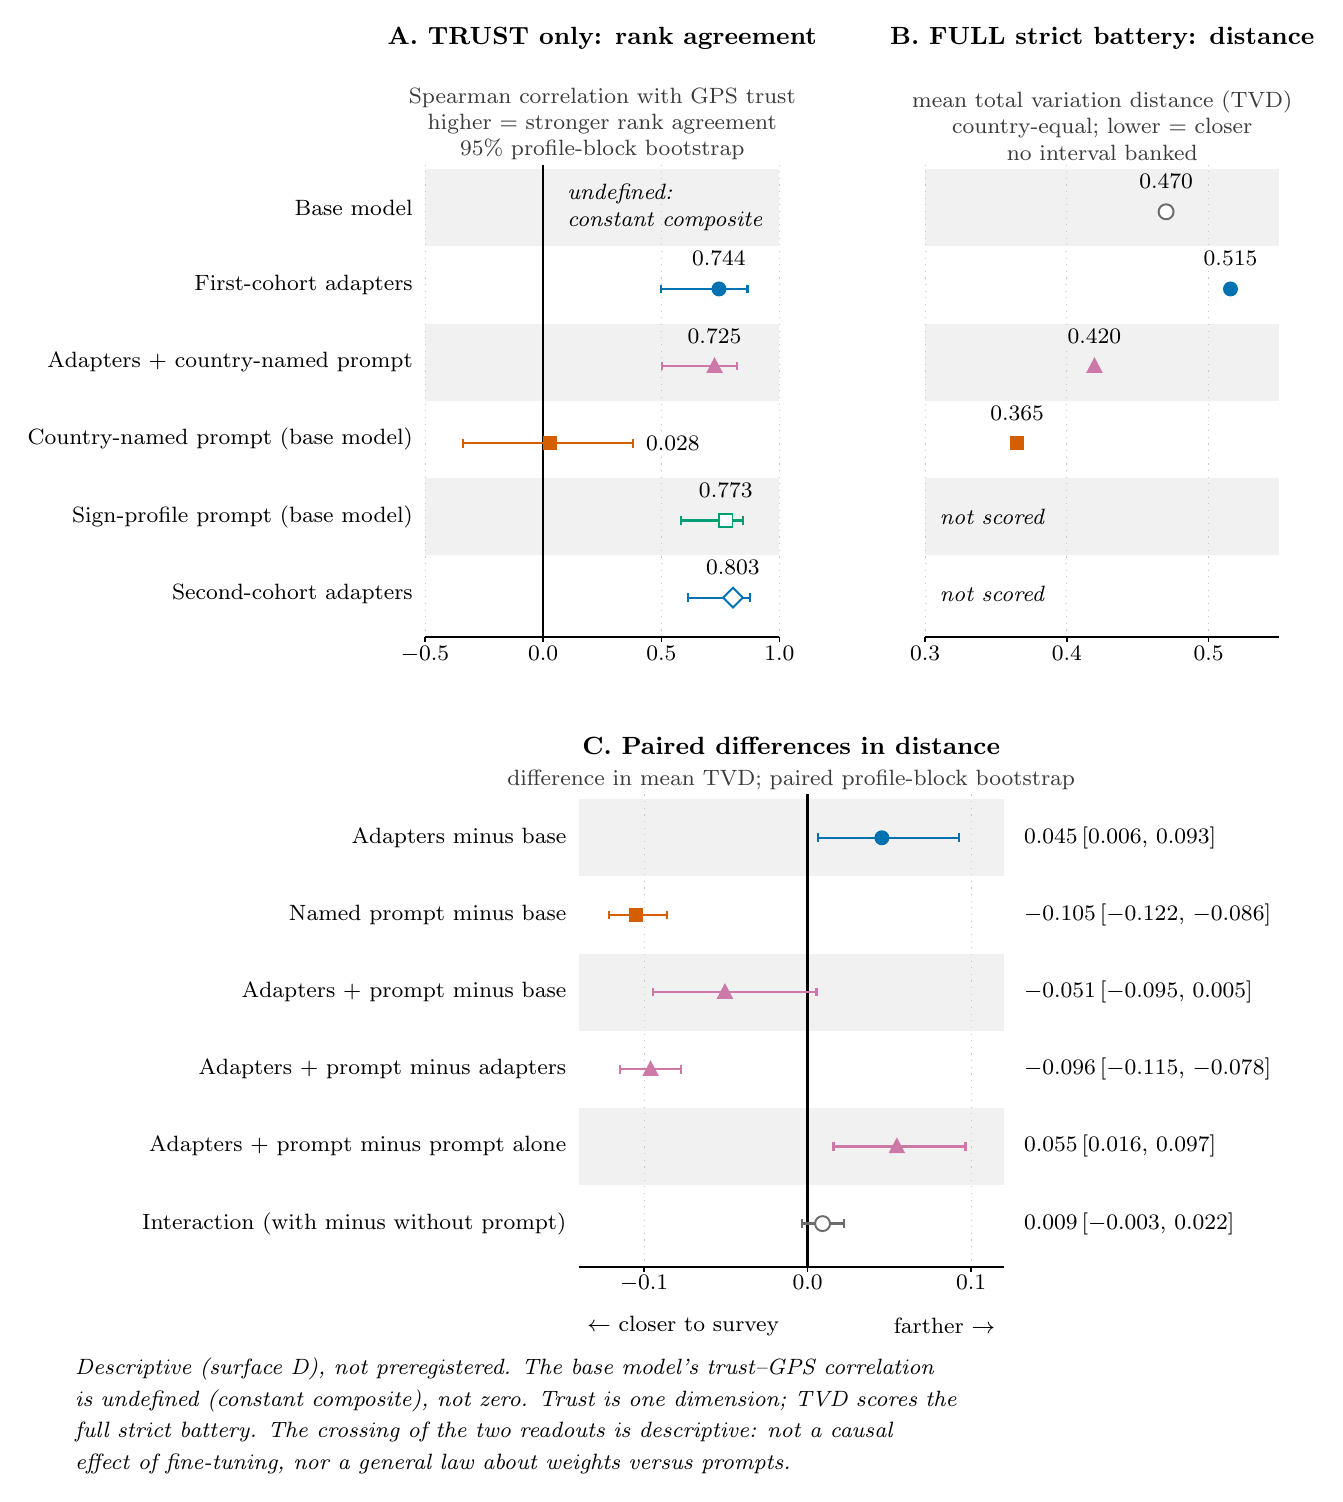
\begin{tikzpicture}[x=1cm,y=1cm,every node/.style={text=black}]
\fill[zebra] (4.450,-1.040) rectangle (8.950,-0.060);
\fill[zebra] (4.450,-3.000) rectangle (8.950,-2.020);
\fill[zebra] (4.450,-4.960) rectangle (8.950,-3.980);
\setpanel{4.45000000000000017763568394002504646778106689453125}{-0.5}{3.000000}
\draw[gridc,line width=0.4pt,dotted] (4.450,0.000)--(4.450,-6.000);
\draw[black,line width=0.5pt] (4.450,-6.000)--(4.450,-6.070);
\node[anchor=north,inner sep=1pt,font=\footnotesize] at (4.450,-6.070) {$-$0.5};
\draw[gridc,line width=0.4pt,dotted] (5.950,0.000)--(5.950,-6.000);
\draw[black,line width=0.5pt] (5.950,-6.000)--(5.950,-6.070);
\node[anchor=north,inner sep=1pt,font=\footnotesize] at (5.950,-6.070) {0.0};
\draw[gridc,line width=0.4pt,dotted] (7.450,0.000)--(7.450,-6.000);
\draw[black,line width=0.5pt] (7.450,-6.000)--(7.450,-6.070);
\node[anchor=north,inner sep=1pt,font=\footnotesize] at (7.450,-6.070) {0.5};
\draw[gridc,line width=0.4pt,dotted] (8.950,0.000)--(8.950,-6.000);
\draw[black,line width=0.5pt] (8.950,-6.000)--(8.950,-6.070);
\node[anchor=north,inner sep=1pt,font=\footnotesize] at (8.950,-6.070) {1.0};
\draw[black,line width=0.5pt] (4.450,-6.000)--(8.950,-6.000);
\draw[black,line width=0.9pt] (5.950,0.000)--(5.950,-6.000);
\node[anchor=south,inner sep=0pt,font=\small\bfseries,align=center] at (6.700,1.450) {A. TRUST only: rank agreement};
\node[anchor=south,inner sep=0pt,font=\footnotesize,text=cS,align=center] at (6.700,0.050) {Spearman correlation with GPS trust\\higher = stronger rank agreement\\95\% profile-block bootstrap};
\fill[zebra] (10.800,-1.040) rectangle (15.300,-0.060);
\fill[zebra] (10.800,-3.000) rectangle (15.300,-2.020);
\fill[zebra] (10.800,-4.960) rectangle (15.300,-3.980);
\setpanel{10.800000000000000710542735760100185871124267578125}{0.3}{18.000000}
\draw[gridc,line width=0.4pt,dotted] (10.800,0.000)--(10.800,-6.000);
\draw[black,line width=0.5pt] (10.800,-6.000)--(10.800,-6.070);
\node[anchor=north,inner sep=1pt,font=\footnotesize] at (10.800,-6.070) {0.3};
\draw[gridc,line width=0.4pt,dotted] (12.600,0.000)--(12.600,-6.000);
\draw[black,line width=0.5pt] (12.600,-6.000)--(12.600,-6.070);
\node[anchor=north,inner sep=1pt,font=\footnotesize] at (12.600,-6.070) {0.4};
\draw[gridc,line width=0.4pt,dotted] (14.400,0.000)--(14.400,-6.000);
\draw[black,line width=0.5pt] (14.400,-6.000)--(14.400,-6.070);
\node[anchor=north,inner sep=1pt,font=\footnotesize] at (14.400,-6.070) {0.5};
\draw[black,line width=0.5pt] (10.800,-6.000)--(15.300,-6.000);
\node[anchor=south,inner sep=0pt,font=\small\bfseries,align=center] at (13.050,1.450) {B. FULL strict battery: distance};
\node[anchor=south,inner sep=0pt,font=\footnotesize,text=cS,align=center] at (13.050,0.050) {mean total variation distance (TVD)\\country-equal; lower = closer\\no interval banked};
\txt{4.300,-0.550}{Base model}{east}{\footnotesize}
\txt{6.250,-0.550}{\shortstack[l]{undefined:\\constant composite}}{west}{\footnotesize\itshape}
\setpanel{10.800000000000000710542735760100185871124267578125}{0.3}{18.000000}
\pval{C9_TVD_base_mean_tvd_country_equal}{0.470046650620059}{-0.600}{h}{cG}
\lbl{C9_TVD_base_mean_tvd_country_equal}{value}{0.470}{}{}{13.861}{-0.350}{south}{zebra}
\txt{4.300,-1.530}{First-cohort adapters}{east}{\footnotesize}
\setpanel{4.45000000000000017763568394002504646778106689453125}{-0.5}{3.000000}
\ival{B2_cohort1_trust_rho}{0.5002088786337604}{0.7441050158009886}{0.8647856310906544}{-1.580}{o}{cA}{solid}
\lbl{B2_cohort1_trust_rho}{value}{0.744}{}{}{8.182}{-1.330}{south}{white}
\setpanel{10.800000000000000710542735760100185871124267578125}{0.3}{18.000000}
\pval{C9_TVD_adapter_mean_tvd_country_equal}{0.5154766417741424}{-1.580}{o}{cA}
\lbl{C9_TVD_adapter_mean_tvd_country_equal}{value}{0.515}{}{}{14.679}{-1.330}{south}{white}
\txt{4.300,-2.510}{Adapters + country-named prompt}{east}{\footnotesize}
\setpanel{4.45000000000000017763568394002504646778106689453125}{-0.5}{3.000000}
\ival{C9_TVD_adapter_persona_trust_gps_profile_block}{0.5045527062375771}{0.7254679523539421}{0.819536884318551}{-2.560}{t}{cD}{solid}
\lbl{C9_TVD_adapter_persona_trust_gps_profile_block}{value}{0.725}{}{}{8.126}{-2.310}{south}{zebra}
\setpanel{10.800000000000000710542735760100185871124267578125}{0.3}{18.000000}
\pval{C9_TVD_adapter_persona_mean_tvd_country_equal}{0.41950116386997005}{-2.560}{t}{cD}
\lbl{C9_TVD_adapter_persona_mean_tvd_country_equal}{value}{0.420}{}{}{12.951}{-2.310}{south}{zebra}
\txt{4.300,-3.490}{Country-named prompt (base model)}{east}{\footnotesize}
\setpanel{4.45000000000000017763568394002504646778106689453125}{-0.5}{3.000000}
\ival{PX_persona_trust_rho}{-0.3386574205085119}{0.02779353374929098}{0.38136686616815824}{-3.540}{s}{cB}{solid}
\lbl{PX_persona_trust_rho}{value}{0.028}{}{}{7.214}{-3.540}{west}{white}
\setpanel{10.800000000000000710542735760100185871124267578125}{0.3}{18.000000}
\pval{C9_TVD_persona_mean_tvd_country_equal}{0.3649046586151852}{-3.540}{s}{cB}
\lbl{C9_TVD_persona_mean_tvd_country_equal}{value}{0.365}{}{}{11.968}{-3.290}{south}{white}
\txt{4.300,-4.470}{Sign-profile prompt (base model)}{east}{\footnotesize}
\setpanel{4.45000000000000017763568394002504646778106689453125}{-0.5}{3.000000}
\ival{PX_signprompt_trust_rho}{0.5836609604950164}{0.7730688066951009}{0.8444114505180651}{-4.520}{q}{cC}{solid}
\lbl{PX_signprompt_trust_rho}{value}{0.773}{}{}{8.269}{-4.270}{south}{zebra}
\txt{10.980,-4.470}{not scored}{west}{\footnotesize\itshape}
\txt{4.300,-5.450}{Second-cohort adapters}{east}{\footnotesize}
\setpanel{4.45000000000000017763568394002504646778106689453125}{-0.5}{3.000000}
\ival{B2_bank2_trust_rho}{0.6145971882846217}{0.8032452595902299}{0.8764662126321977}{-5.500}{d}{cA}{solid}
\lbl{B2_bank2_trust_rho}{value}{0.803}{}{}{8.360}{-5.250}{south}{white}
\txt{10.980,-5.450}{not scored}{west}{\footnotesize\itshape}
\fill[zebra] (6.400,-9.040) rectangle (11.800,-8.060);
\fill[zebra] (6.400,-11.000) rectangle (11.800,-10.020);
\fill[zebra] (6.400,-12.960) rectangle (11.800,-11.980);
\setpanel{6.4000000000000003552713678800500929355621337890625}{-0.14}{20.769231}
\draw[gridc,line width=0.4pt,dotted] (7.231,-8.000)--(7.231,-14.000);
\draw[black,line width=0.5pt] (7.231,-14.000)--(7.231,-14.070);
\node[anchor=north,inner sep=1pt,font=\footnotesize] at (7.231,-14.070) {$-$0.1};
\draw[gridc,line width=0.4pt,dotted] (9.308,-8.000)--(9.308,-14.000);
\draw[black,line width=0.5pt] (9.308,-14.000)--(9.308,-14.070);
\node[anchor=north,inner sep=1pt,font=\footnotesize] at (9.308,-14.070) {0.0};
\draw[gridc,line width=0.4pt,dotted] (11.385,-8.000)--(11.385,-14.000);
\draw[black,line width=0.5pt] (11.385,-14.000)--(11.385,-14.070);
\node[anchor=north,inner sep=1pt,font=\footnotesize] at (11.385,-14.070) {0.1};
\draw[black,line width=0.5pt] (6.400,-14.000)--(11.800,-14.000);
\draw[black,line width=0.9pt] (9.308,-8.000)--(9.308,-14.000);
\node[anchor=south,inner sep=0pt,font=\small\bfseries,align=center] at (9.100,-7.500) {C. Paired differences in distance};
\node[anchor=south,inner sep=0pt,font=\footnotesize,text=cS,align=center] at (9.100,-7.950) {difference in mean TVD; paired profile-block bootstrap};
\txt{6.250,-8.550}{Adapters minus base}{east}{\footnotesize}
\setpanel{6.4000000000000003552713678800500929355621337890625}{-0.14}{20.769231}
\ival{C9_TVD_adapter_minus_base_profile_block}{0.006169716953512208}{0.04542999115408338}{0.09272260519372265}{-8.550}{o}{cA}{solid}
\lblci{C9_TVD_adapter_minus_base_profile_block}{0.045}{0.006}{0.093}{12.050}{-8.550}{west}
\txt{6.250,-9.530}{Named prompt minus base}{east}{\footnotesize}
\setpanel{6.4000000000000003552713678800500929355621337890625}{-0.14}{20.769231}
\ival{C9_TVD_persona_minus_base_profile_block}{-0.12158126165639337}{-0.10514199200487398}{-0.08606035054516069}{-9.530}{s}{cB}{solid}
\lblci{C9_TVD_persona_minus_base_profile_block}{$-$0.105}{$-$0.122}{$-$0.086}{12.050}{-9.530}{west}
\txt{6.250,-10.510}{Adapters + prompt minus base}{east}{\footnotesize}
\setpanel{6.4000000000000003552713678800500929355621337890625}{-0.14}{20.769231}
\ival{C9_TVD_adapter_persona_minus_base_profile_block}{-0.09453081764312539}{-0.05054548675008909}{0.00548412981330979}{-10.510}{t}{cD}{solid}
\lblci{C9_TVD_adapter_persona_minus_base_profile_block}{$-$0.051}{$-$0.095}{0.005}{12.050}{-10.510}{west}
\txt{6.250,-11.490}{Adapters + prompt minus adapters}{east}{\footnotesize}
\setpanel{6.4000000000000003552713678800500929355621337890625}{-0.14}{20.769231}
\ival{C9_TVD_adapter_persona_minus_adapter_profile_block}{-0.11452277939054879}{-0.09597547790417249}{-0.07763268990263332}{-11.490}{t}{cD}{solid}
\lblci{C9_TVD_adapter_persona_minus_adapter_profile_block}{$-$0.096}{$-$0.115}{$-$0.078}{12.050}{-11.490}{west}
\txt{6.250,-12.470}{Adapters + prompt minus prompt alone}{east}{\footnotesize}
\setpanel{6.4000000000000003552713678800500929355621337890625}{-0.14}{20.769231}
\ival{C9_TVD_adapter_persona_minus_persona_profile_block}{0.01587128110326034}{0.05459650525478486}{0.09662035133703001}{-12.470}{t}{cD}{solid}
\lblci{C9_TVD_adapter_persona_minus_persona_profile_block}{0.055}{0.016}{0.097}{12.050}{-12.470}{west}
\txt{6.250,-13.450}{Interaction (with minus without prompt)}{east}{\footnotesize}
\setpanel{6.4000000000000003552713678800500929355621337890625}{-0.14}{20.769231}
\ival{C9_TVD_interaction_profile_block}{-0.0032999105110756164}{0.00916651410070148}{0.022368632285632302}{-13.450}{h}{cG}{solid}
\lblci{C9_TVD_interaction_profile_block}{0.009}{$-$0.003}{0.022}{12.050}{-13.450}{west}
\txt{6.504,-14.750}{$\leftarrow$ closer to survey}{west}{\footnotesize}
\txt{11.696,-14.750}{farther $\rightarrow$}{east}{\footnotesize}
\txt{0.000,-15.300}{Descriptive (surface D), not preregistered. The base model's trust--GPS correlation}{west}{\footnotesize\itshape}
\txt{0.000,-15.700}{is undefined (constant composite), not zero. Trust is one dimension; TVD scores the}{west}{\footnotesize\itshape}
\txt{0.000,-16.100}{full strict battery. The crossing of the two readouts is descriptive: not a causal}{west}{\footnotesize\itshape}
\txt{0.000,-16.500}{effect of fine-tuning, nor a general law about weights versus prompts.}{west}{\footnotesize\itshape}
\end{tikzpicture}
\end{document}
